
\documentclass[11pt, letterpaper]{article}
%\usepackage{bookmark}
\usepackage[a4paper,margin=2cm]{geometry}
\usepackage[]{graphicx}
\usepackage{bm}
\usepackage[strings]{underscore}
\usepackage{apacite}
\graphicspath{ {./Images} }

\begin{document}
\begin{titlepage}
	\title{Modeling and Lighting Interior Spaces using Reflected Natural Light}
	\author{Noah Alexiou}
	\date{\today}
	
	\maketitle
	\centering
	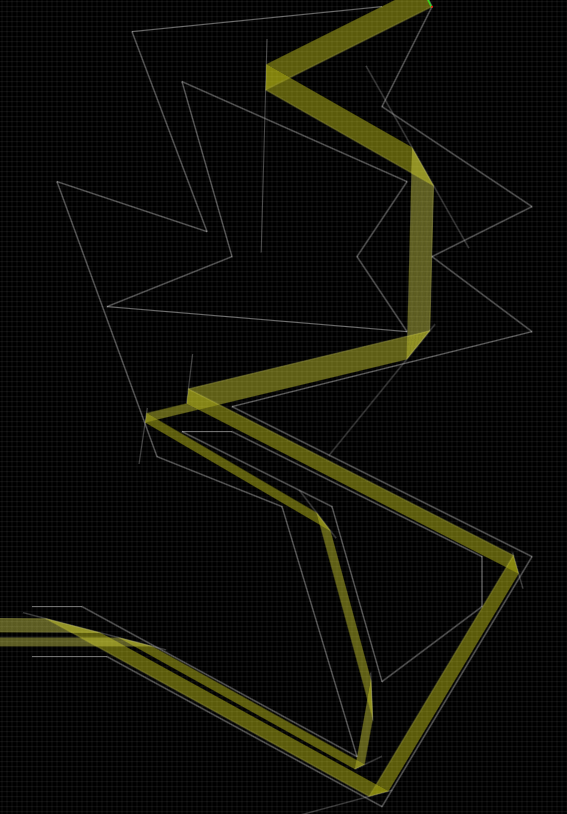
\includegraphics[width=14cm]{cave2.png}
	
\end{titlepage}

\newpage
\tableofcontents


\newpage

\section{Introduction}


\subsection{Premise}
- Study aims to find optimal mirror placement for minimum decrease in intensity as light travels throughout the cave. This will be achieved by mapping the cave's geometry and simulating the travel of light throughout the cave as a vector. 




\subsection{Assumptions} 
\par
In Order for a solution to be formed, a set of conditions must be assumed .
\begin{itemize}

	\item The given specifications do not list whether the cave is horizontal or vertical, so it will be assumed that the cave described is traversed horizontally. This also implies that in all diagrams and depictions, the cave is being viewed from a 'top-down' view.
	
	\item The mirrors and walls of the cave are perfectly parallel to the floor of the cave and extend upwards with an undefined height. This simplifies modeling and can easily be altered to fit revised specifications, such as only needing to light the floor of the cave.
	

	\item Either light does not decrease in intensity or increase in area according to the inverse square law, or the change is negligible. The suns rays have traveled so far that they can be considered effectively parallel and therefore will not diverge. 
	\cite{yasuda_2024_why}
		
	\item mirrors will reflect light across their entire surface, even at the very tips of their edges. 
	
	\item mirrors are perfectly flat and do not distort or affect light beams in any other way than reflecting them
	
	\item While the entry vector has no width, it will be assumed that light will enter the cave through the entire entrance. Each point along the entrance will be the beginning of its own vector, with equal direction to the entry vector. This assumption allows the 
	
		
	\item Light will enter the cave parallel to the ground and of equal intensity from floor to ceiling.
	

\end{itemize}

\subsection{Observations}
\par
\begin{itemize}
\item Vectors can be modeled on the Cartesian plane and translated without affecting their properties. 

\item Light can be modeled as a relative position vector with origin at a mirror surface

\item Light will reflect so that $\textrm{angle  of incidence} = \textrm{angle of refraction}$.

\item Light will not diverge however contaminants in the air may decrease the intensity of light. Distance light travels in cave must me minimized

\item Mirrors are not perfect and will only reflect a portion of light that hits them. 

\item Only the edges of each beam of light need to be found as any light that is within a beam will be traveling the same direction as the light at the edges. This allows intersections with mirrors and cave walls to be found without introducing unnecessary calculations. 

\item  Since it is assumed that light will not diverge. the maximum size a mirror must be to reflect all the light hitting it will be 2 units, or the size of the cave's entrance. 

\item Clearly paths are not wide enough for a beam of 2 units to pass through them without a significant number of mirrors, therefore the beam may have to be split in order for them to be passed through the cave efficiently 

\item in the case of the beam being split, the edges of each beam will be found and each considered the new edge for the split path

\end{itemize}





\subsection{Translation}
\par 

\begin{itemize}

\item  \textbf{move this to translation} This angle can be found by first calcualting the \textit{dot product} and then using it to find the acute angle between the vecotrs. Using the calculated acute angles, subtract the 	

\item	As mentioned, mirrors are not perfect. The amount of light lost when a reflection occurs can be modelded as an exponential, $I=\textrm{Efficiency}^x$, where I is intensity of light, n is the number of mirrors, and efficiency is the percentage efficiency of the mirror in decimal form. Clearly  adding more mirrors will lead to exponential losses in intensity.

\item Vector addition can be used to join each given vector and form the walls of the cave and the obstacles

\item Used Excel to do vector addition

\item Took points from excel and inserted them as separate $x$ and $y$ list in desmos

\item Graphed each point on list and joined points with lines.

\item Imported Lists as points in phydemo.app

\item Used the given lists and entry vector to draft a path through the cave

\item  clearly some sections of the cave are too narrow so split beam. More distance but drastic reduction in mirrors while maintianing full beam area

\item translate mirrors from phyapp demo into lists of points for desmos

\item graph linear equations from the lines formed between points (i.e. the locations of mirrors) and find intersections with initial beam of light

\item  trim mirrors to minimum size

\item calculate angle of reflected beam 

\item repeat for all items and alter angles if a collision with the walls of the cave or an obstacle occurs

\item if a colission occurs, then tweak mirror angle to correct and repeat

\item verify light exiting cave is aligned with exit vector by measusing angle against entry vector
\end{itemize}


\par 


\section{Solve}

\par 
what do i put here exactly?

\section{Evaluate and Verify}



\subsection{Extentions}
\begin{itemize}
\item Use of Lenses	or curved mirrors to focus or manipulate light 
\item Quantification of intensity and how factors such as distance and number of mirrors affect it in order to further optimize for maximum intensity. 
\item use of algortihms to find the most mathematically correct solution.
\item Conversion into an optimisation problem
	
\end{itemize}



\subsection{Reasonableness}
\begin{itemize}
\item verified that solution was valid through visual inspection in desmos and through checking angle of exit vector
\end{itemize}

\subsection{Strengths and Limitations of Solution}
\subsubsection{Strengths}
\begin{itemize}
\item No light was lost through absoption into the cave walls
\item the solution used the minimum amount of mirrors found to be required
\end{itemize}
\subsubsection{Limitations}
\begin{itemize}
\item beams never come together as they were at the entrance. 2 seperate beams come out. they do go out the exit though

\item Beams are not perfectly parralel with exit vector when they exit. 

\item Low tolerance for error in mirror placement in case of physical instalation, which is imminent considering the context of the task

\item Solution is not very refined or automated. There are many steps that require manual intervention and this process is easily repeatable for other cave geometries

\end{itemize}
\section{Conclusion}


 \newpage
 \bibliographystyle{apacite}
 \bibliography{References}

\end{document}
